\PassOptionsToPackage{svgnames}{xcolor}
\documentclass[12pt]{article}



\usepackage[margin=1in]{geometry}  
\usepackage{algorithm,algpseudocode}
\newcommand{\vars}{\texttt}
\newcommand{\func}{\textrm}
\usepackage{graphicx}             
\usepackage{amsmath}              
\usepackage{amsfonts}
\usepackage{framed}               
\usepackage{amssymb}
\usepackage{array}
\usepackage{amsthm}
\usepackage{multirow}
\usepackage[nottoc]{tocbibind}
\usepackage{bm}
\usepackage{enumitem}
\usepackage{tikz}
\usepackage{pdfpages}
\usepackage{tabularx}
\algdef{SE}[SUBALG]{Indent}{EndIndent}{}{\algorithmicend\ }%
\algtext*{Indent}
\algtext*{EndIndent}
\newcolumntype{C}[1]{>{\centering\let\newline\\\arraybackslash\hspace{0pt}}m{#1}}
\newcommand\norm[1]{\left\lVert#1\right\rVert}
\setlength{\parindent}{0cm}
\setlength{\parskip}{0em}
\newcommand{\ind}{\hspace*{15pt}}
\newcommand{\Lim}[1]{\raisebox{0.5ex}{\scalebox{0.8}{$\displaystyle \lim_{#1}\;$}}}
\newtheorem{definition}{Definition}[section]
\newtheorem{theorem}{Theorem}[section]
\newtheorem{notation}{Notation}[section]
\theoremstyle{definition}
\DeclareMathOperator{\arcsec}{arcsec}
\DeclareMathOperator{\arccot}{arccot}
\DeclareMathOperator{\arccsc}{arccsc}
\DeclareMathOperator{\spn}{Span}
\setcounter{tocdepth}{1}
\begin{document}
\title{Revision notes - CS3243}
\author{Ma Hongqiang}
\maketitle
\tableofcontents

\clearpage
%\twocolumnt
\section{Introduction}
\subsection{Definition of Artificial Intelligence(AI)}
Artificial Intelligence has the following defining behaviour:
\begin{enumerate}
	\item Think like a human
	\item Think rationally
	\item Act like a human
	\item Act rationally
\end{enumerate}
Turing test can be used to test (3) whether AI is acting humanly.\\
For (2), there are problems like
\begin{itemize}
	\item Can \textbf{all intelligent} behaviour be captured by logical rules?
	\item Due to \textbf{computational issues}, a logical solution in principle does not translate to practice.
\end{itemize}
To (4) act rationally, we define rational behaviour as doing the "right thing", whose definition is subjective:
\begin{itemize}
	\item Best for whom?
	\item What to optimise?
	\item What information is available?
	\item Unintended effects?
\end{itemize}
\subsection{Rational Agents}
\begin{definition}[Agent]
\hfill\\\normalfont An agent is an entity that \textbf{perceives and acts}.\\Formally, an agent is a function $f$ from percept histories to actions, i.e.,
\[
f:P^\ast\to A
\]
\end{definition}
Ideally, we seek the best-performing agent for a certain task subject to computation limits.
\clearpage
\section{Intelligent Agents}
From the previous section, we know that agents are anything that can be viewed as \textbf{perceiving} its \textbf{environment} through \textbf{sensors}; \textbf{acting} upon that environment through \textbf{actuators}.\\
In other words, sensors and actuators are two interfaces through which agent program interacts with the environment. \\So an agent comprises of both \textbf{architecture} and \textbf{program}.
\begin{definition}[Rational Agent]
\hfill\\\normalfont A rational agent is an agent that maximise agent success based on what it can perceive and the actions it can perform.\\The agent success is judged by a performance measure, defined as an objective criterion for meansuring success of an agent's behaviour.
\end{definition}
Rational agents behave in a way such that for each possible percept sequence, it selects an action that is expected to maximise its performance measure, given the evidence provided by the percept sequence and whatever built-in knowledge the agent has.\\
\textbf{Remark}: Rationality $\neq$ omniscience. Agents can perform \textbf{exploration} that help them gather useful information, before \textbf{exploitation} of known information.
\begin{definition}[Autonomous Agent]
\hfill\\\normalfont An agent is \textbf{autonomous} if its behaviour is determined by its own experience, with ability to learn and adapt.
\end{definition}
\subsection{Task Environment}
To specify the task environment for the design of intelligent agent, we focuses on \textbf{PEAS}:
\begin{itemize}
	\item Performance measure
	\item Environment
	\item Actuators
	\item Sensors
\end{itemize}
There are several properties of task environment listed down in the following table. Detailed explanation in the next page.
\begin{table}[h]
\centering
\begin{tabular}{|l|l|}
\hline
\textbf{Properties}&\textbf{Complement}\\\hline
Fully observable&Partially observable\\\hline
Deterministic&Stochastic\\\hline
Episodic&Sequential\\\hline
Static&Dynamic\\\hline
Discrete&Continuous\\\hline
Single agent&Multi-agent\\\hline
\end{tabular}
\end{table}
\clearpage
\textbf{Fully observable} means sensors provide access to the complete state of the environment at each point in time.\\
\textbf{Deterministic} means the next state of the environment is completely determinedby the current state and the action executed by the agent.\\
\textbf{Episodic} means (1) the agent’s experience is divided into atomic “episodes” (each episode consists of the agent perceiving and then performing a single action); and (2) the choice of action in each episode does not depend on actions in past episodes.\\
\textbf{Static} means the environment is unchanged while an agent is deliberating.\\
\textbf{Discrete} means there exists a finite number of distinct states, percepts, and actions.\\
\textbf{Single agent} means there is only one agent operating by iteself in an environment.
\subsection{Implementation of Agent Function}
Since an agent is completely specified by the \textbf{agent function} which maps percept sequences to actions, we need to ensure one, or a small equivalence class of it is \textbf{rational}.\\
\begin{definition}[Table-Lookup Agent]
\hfill\\\normalfont Table-lookup agent is defined by the following agent function:
\begin{algorithm}[h]
\begin{algorithmic}
\Function{Table-Driven-Agent}{\vars{percept}}\;\Return\vars{action}
	\Indent
	\func{static}:\begin{tabular}{l} \vars{percepts}, a sequence initially empty\\
	\vars{table}, a table of actions, indexed by percept sequences, fully specified
	\end{tabular}
	\EndIndent
	\State append \vars{percept} to the end of \vars{percepts}
	\State \vars{action}$\leftarrow$ \Call{LookUp}{\vars{percepts},\vars{table}}
\EndFunction
\end{algorithmic}
\end{algorithm}
\end{definition}
It has the following drawbacks:
\begin{itemize}
	\item Huge table to store
	\item Take a long time to build the table
	\item No autonomy: impossible to learn all correct table entries from experience
	\item No guidance on filling the correct table entries
\end{itemize}
\subsection{Agent Types}
There are 4 basic types of agents in order of \textit{increasing} generality:
\begin{itemize}
	\item Simple reflex agent
	\item Model-based reflex agent
	\item Goal-based agent
	\item Utility-based agent
\end{itemize}
\subsubsection{Simple Reflex Agent}
A simple reflex agent selects actions based on the \textbf{current} percept, ignoring rest of percept history. \\
What the world is like now: \texttt{interpret\_input}; what action I should do now: \texttt{rule\_match}
\begin{figure}[h]
\centering
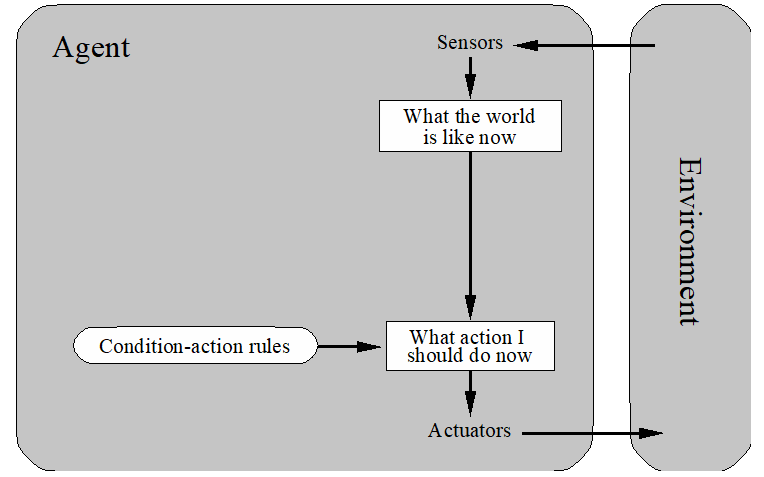
\includegraphics[width = 0.7\textwidth]{2_1.png}
\end{figure}
It is considered a computationally cheap agent program, used to achieve instantaneous reaction.
\subsubsection{Model-based Reflex Agent}
A model-based reflex agent handles partial observability by keeping track of environment state it cannot perceive now. Therefore, it depends on percept history.\\
What the world is like now: \texttt{update\_state}; what action I should do now: \texttt{rule\_match}
\begin{figure}[h]
\centering
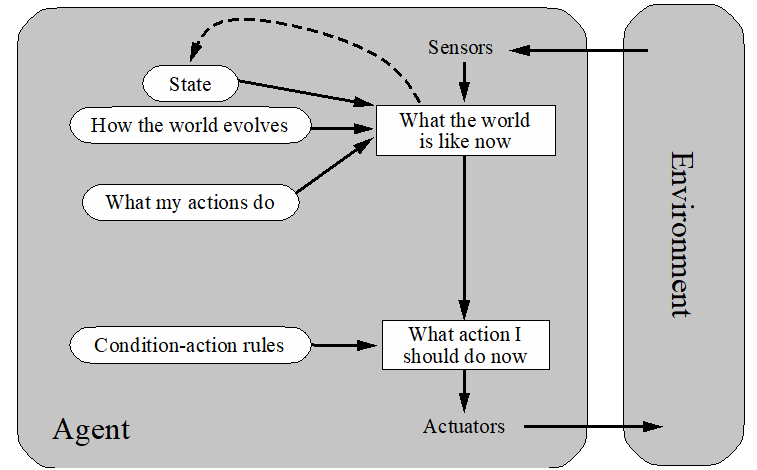
\includegraphics[width = 0.7\textwidth]{2_2.png}
\end{figure}
\subsubsection{Goal-based Agent}\
A goal-based agent has a goal which is used to describe which states are desirable. It also considers next state: whether action $A$ result in a next state which achieves the goal?
\begin{figure}[h]
\centering
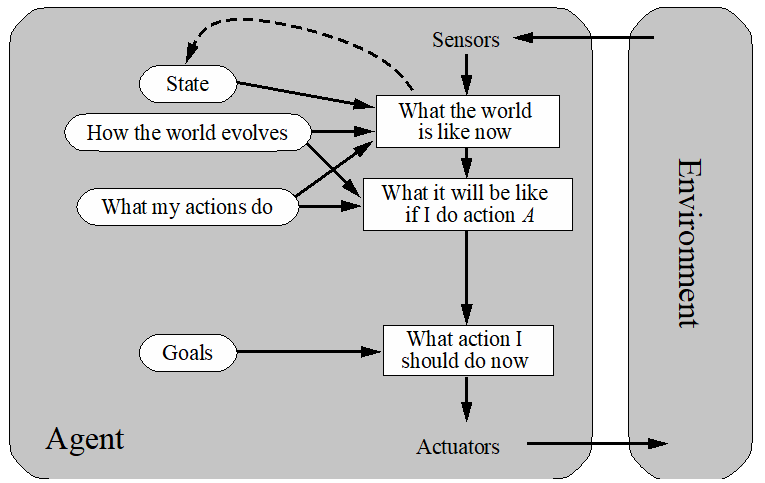
\includegraphics[width = 0.7\textwidth]{2_3.png}
\end{figure}
While it is less efficient, it is more flexible since the goal can be easily changed without recoding all condition-action rules.
\subsubsection{Utility-based Agent}
A utlity-based agent can handle partially observable and stochastic properties very well using expectation.
\begin{figure}[h]
\centering
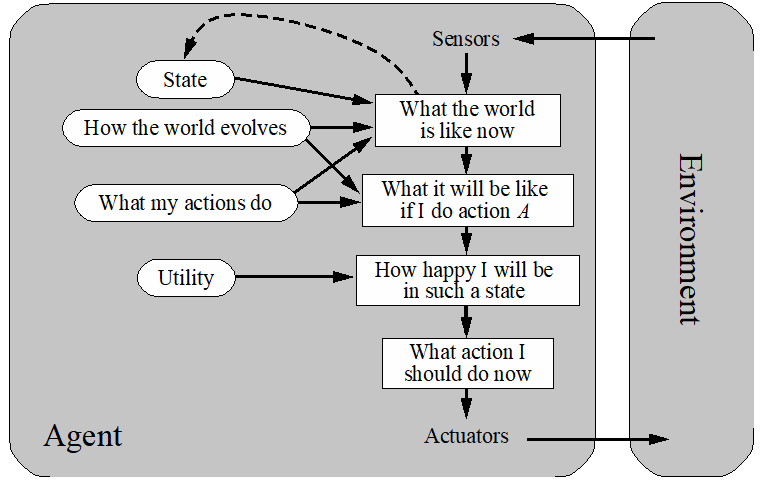
\includegraphics[width = 0.7\textwidth]{2_4.png}
\end{figure}
\subsubsection{Learning Agent}
Learning agent is to operate in initially unknown environments and perform better than other agents with prior knowledge.
\begin{figure}[h]
\centering
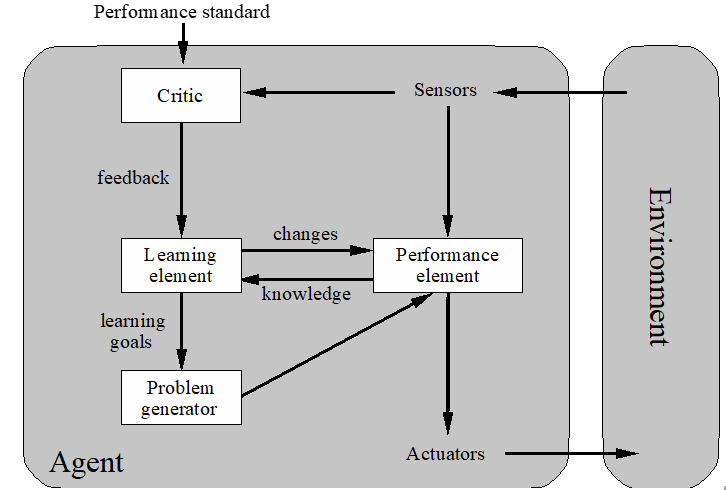
\includegraphics[width = 0.7\textwidth]{2_5.png}
\end{figure}
Components in the learning agent include
\begin{itemize}
\item Performance element: selects the external actions
\item Learning element: improves agent to perform better
\item Critic: provides feedback on how well the agent is doing
\item Problem generator: suggests explorative actions that will lead to new, informative (but not necessarily better) experiences
\end{itemize}
\subsection{Exploitation vs. Exploration}
An agent operating in the real world must choose between
\begin{enumerate}
	\item maximizing its expected utility according to its current knowledge about the world; and 
	\item trying to learn more about the world since this may improve its future gains. 
\end{enumerate}
This problem is known as the trade-off between exploitation and exploration.
\clearpage
\section{Uninformed Search}
In this section, searching is conducted in fully \textbf{observable}, \textbf{deterministic} and \textbf{discrete} environment.\\
Under these conditions, the solution to any problem is a fixed sequence of actions.
\subsection{Problem Formulation}
Usually the problem needs to be modelled before searching can be conducted. \\ 
A problem can be defined formally by five components:
\begin{itemize}
	\item \textbf{Initial state} that the agents starts in
	\item A description of possible \textbf{actions} available to the agent
	\item \textbf{Transition model}, i.e., a description of what each action does 
	\item A goal test which determines whether a state $S$ is a goal state. The goal states can be
\begin{itemize}
	\item explicitly specified as a set, e.g., $\{InWork\}$, or
	\item implicit function, e.g., $isCheckMate(s)$.
\end{itemize}
\item A \textbf{Path cost} function that assigns a numeric cost to each path.
\end{itemize}
\begin{definition}[Cost Function and Path Cost]
\hfill\\\normalfont A cost function from state $s$ to $s'$ under action $a$ is denoted as
\[
c(s, a, s')
\]
For this section, cost is non-negative, i.e., $c\geq 0$.\\
Path cost is usually additive and is calculated from $\sum_{c\in \text{Path}}c$.
\end{definition}
Below is a simple problem-solving agent.\\
\textbf{function} \textsc{SIMPLE-PROBLEM-SOLVING-AGENT}(\textit{percept}) \textbf{returns} an action\\
\ind persistent: \textit{seq}, an action sequence, initially empty\\
\ind\ind\ind\ind \textit{state}, somne description of the current world state\\
\ind\ind\ind\ind \textit{goal} , a goal, initially null\\
\ind\ind\ind\ind \textit{problem}, a problem formulation\\
\ind state$\leftarrow$ \textsc{UPDATE-STATE}(\textit{state}, \textit{percept})\\
\ind \textbf{if} \textit{seq} is empty \textbf{then}\\
\ind\ind \textit{goal} $\leftarrow$\textsc{FORMULATE-GOAL}(\textit{state})\\
\ind\ind \textit{problem} $\leftarrow$\textsc{FORMULATE-PROBLEM}(\textit{state}, \textit{goal})\\
\ind\ind \textit{seq} $\leftarrow$\textsc{SEARCH}(\textit{problem})\\
\ind\ind \textbf{if} \textit{seq} = \textit{failure} \textbf{then return} a null action\\
\ind \textit{action} $\leftarrow$\textsc{FIRST}(\textit{seq})\\
\ind \textit{seq} $\leftarrow$\textsc{REST}(\textit{seq})\\
\ind \textbf{return} action

In consideration of limited computation resources, state space has to be abstracted, where
\begin{itemize}
	\item state is abstracted to set of real states
	\item action is abstracted to complex combination of real actions
	\item solutions is abstracted to set of real paths
\end{itemize}
Such abstraction needs to be both \textbf{valid} and \textbf{useful}.
\subsection{Tree Search Algorithms}
\begin{definition}[Tree Search Algorithm]
\hfill\\\normalfont Below is the general tree search algorithm.\\
\textbf{function} \textsc{TREE-SEARCH}(\textit{problem}) \textbf{returns} a solution, or failure\\
\ind initialize the frontier using the initial state of \textit{problem}\\
\ind \textbf{loop do}\\
\ind \ind \textbf{if} the frontier is empty \textbf{then return} failure\\
\ind \ind choose a leaf node and remove it from the frontier\\
\ind \ind \textbf{if} the node contains a goal state \textbf{then return} the corresponding solution\\
\ind \ind expand the chosen node, adding the resulting nodes to the frontier
\end{definition}
\textbf{Remark}: In tree search, the exploration is \textbf{memoryless}, so \textbf{redundant paths} are unavoidable.
\subsection{Graph Search Algorithms}
\begin{definition}[Graph Search Algorithm]
\hfill\\\normalfont Below is the general graph search algorithm. It augments the tree search algorithm with a \textbf{explored set}.\\
\textbf{function} \textsc{GRAPH-SEARCH}(\textit{problem}) \textbf{returns} a solution, or failure\\
\ind initialize the frontier using the initial state of \textit{problem}\\
\ind \textbf{initialize the explored set to be empty}\\
\ind \textbf{loop do}\\
\ind \ind \textbf{if} the frontier is empty \textbf{then return} failure\\
\ind \ind choose a leaf node and remove it from the frontier\\
\ind \ind \textbf{if} the node contains a goal state \textbf{then return} the corresponding solution\\
\ind \ind \textbf{add the node to the explored set}\\
\ind \ind expand the chosen node, adding the resulting nodes to the frontier\\
\ind \ind \ind \textbf{only if not in the frontier or explored set}
\end{definition}
\textbf{Nodes} in graph search algorithms usually contain the following information:
\begin{itemize}
	\item \textbf{State} to which the node corresponds
	\item \textbf{Parent} node which generates this node
	\item \textbf{Action} that was applied to the parent to generate this node
	\item \textbf{Path Cost} $g(n)$ of the path from the initial state to the node
\end{itemize}
\textbf{Remark}: Search strategies are mostly determined by the \textbf{order of node expansion}.\\
The performance of search algorithms can be measured in
\begin{itemize}
\item Completeness: Solution guaranteed
\item Optimality: Optimal solution found
\item Time complexity
\item Space complexity
\end{itemize}
\begin{definition}[Parameters for Analysis]
\hfill\\\normalfont We define
\begin{itemize}
	\item $b$: maximum number of successors of any node
	\item $d$ depth of shallowest goal node, and
	\item $m$: maximum depth of search tree
\end{itemize}
to assist the measurement of performance.
\end{definition}
Next, we look into 4 \textbf{uninformed search}, mearning that the strategies have no additional information about states beyond that provided in the problem definition.
\subsubsection{Breadth First Search}
Breadth-first search is a simple strategy in which the root node is expanded first, then all the successors of the root node are expanded next, then their successors, and so on. In general, all the nodes are expanded at a given depth in the search tree before any nodes at the next level are expanded.\\
\textbf{function} \textsc{BREADTH-FIRST-SEARCH}(\textit{problem}) \textbf{returns} a solution, or failure\\
\ind \textit{node}$\leftarrow$a node with \textsc{STATE} = \textit{problem}.\textsc{INITIAL-STATE}, \textsc{PATH-COST} = 0\\
\ind \textbf{if} \textit{problem}.\textsc{GOAL-TEST}(\textit{node}.\textsc{STATE}) \textbf{then return} \textsc{SOLUTION}(\textit{node})\\
\ind \textit{frontier} $\leftarrow$a FIFO queue with \textit{node} as the only element\\
\ind \textit{explored} $\leftarrow$an empty set\\
\ind \textbf{loop do}\\
\ind \ind \textbf{if} EMPTY?( \textit{frontier}) \textbf{then return} failure\\
\ind \ind \textit{node}$\leftarrow$POP( \textit{frontier} ) /* chooses the shallowest node in \textit{frontier} */\\
\ind \ind add \textit{node}.\textsc{STATE} to \textit{explored}\\
\ind \ind \textbf{for each} \textit{action} \textbf{in} \textit{problem}.\textsc{ACTIONS}(\textit{node}.\textsc{STATE}) \textbf{do}\\
\ind \ind \ind child $\leftarrow$\textsc{CHILD-NODE}(\textit{problem}, \textit{node}, \textit{action})\\
\ind \ind \ind \textbf{if} \textit{child}.\textsc{STATE} is not in \textit{explored} or \textit{frontier} \textbf{then}\\
\ind \ind \ind \ind \textbf{if} \textit{problem}.\textsc{GOAL-TEST}(\textit{child}.\textsc{STATE}) \textbf{then return} \textsc{SOLUTION}(\textit{child} )\\
\ind\ind\ind\ind\textit{frontier} $\leftarrow$\textsc{INSERT}(\textit{child} , \textit{frontier} )\\

Above is breadth-first search on a graph.\\
\textbf{Remark}: Breadth-first search is optimal only if step costs are all identical.
\subsubsection{Uniform-cost Search}
Uniform-cost search expands on the idea of BFS, with frontier implemented by a priority queue.\\
With this modification, UCS is in general optimal.
\textbf{function} \textsc{UNIFORM-COST-SEARCH}(\textit{problem}) \textbf{returns} a solution, or failure\\
\ind \textit{node} $\leftarrow$a node with \textsc{STATE} = \textit{problem}.\textsc{INITIAL-STATE}, \textsc{PATH-COST} = 0\\
\ind \textit{frontier} $\leftarrow$a priority queue ordered by \textsc{PATH-COST}, with \textit{node} as the only element\\
\ind \textit{explored} $\leftarrow$an empty set\\
\ind \textbf{loop do}\\
\ind \ind \textbf{if} EMPTY?(\textit{frontier}) \textbf{then return} failure\\
\ind \ind \textit{node}$\leftarrow$POP(\textit{frontier}) /* chooses the lowest-cost node in \textit{frontier} */\\
\ind \ind \textbf{if} \textit{problem}.\textsc{GOAL-TEST}(\textit{node}.\textsc{STATE}) \textbf{then return} \textsc{SOLUTION}(\textit{node})\\
\ind \ind add \textit{node}.\textsc{STATE} to explored\\
\ind \ind \textbf{for each} \textit{action} in \textit{problem}.\textsc{ACTIONS}(\textit{node}.\textsc{STATE}) \textbf{do}\\
\ind \ind \ind \textit{child} $\leftarrow$\textsc{CHILD-NODE}(\textit{problem},\textit{node}, \textit{action})\\
\ind \ind \ind \textbf{if} \textit{child}.\textsc{STATE} is not in \textit{explored} or \textit{frontier} \textbf{then}\\
\ind \ind \ind \ind \textit{frontier} $\leftarrow$\textsc{INSERT}(\textit{child} , \textit{frontier} )\\
\ind \ind \ind else if \textit{child}.\textsc{STATE} is in \textit{frontier} with higher \textsc{PATH-COST} then\\
\ind \ind \ind \ind replace that \textit{frontier} node with \textit{child}\\

\subsubsection{Depth First Search}
Depth-first search always expands the deepest node in the current frontier of the search tree. The search proceeds immediately to the deepest level of the search tree, where the nodes have no successors. As those nodes are expanded, they are dropped from the frontier, so then the search “backs up” to the next deepest node that still has unexplored successors.\\
Its frontier is implemented using a stack.\\
\subsubsection{Depth-limited Search}
DFS may fail if there is infinite state spaces. This can be solved using Depth Limited Search, by supplying DFS with a predetermined depth limit $l$. That is, nodes at depth $l$ are treated as if they have no successors.\\
\textbf{function} \textsc{DEPTH-LIMITED-SEARCH}(\textit{problem}, \textit{limit} ) \textbf{returns} a solution, or failure/cutoff\\
\ind \textbf{return} \textsc{RECURSIVE-DLS}(\textsc{MAKE-NODE}(\textit{problem}.\textsc{INITIAL-STATE}), \textit{problem}, \textit{limit})\\

\textbf{function} \textsc{RECURSIVE-DLS}(\textit{node}, \textit{problem}, \textit{limit} ) \textbf{returns} a solution, or failure/cutoff\\
\ind \textbf{if} \textit{problem}.\textsc{GOAL-TEST}(\textit{node}.\textsc{STATE)} \textbf{then return} \textsc{SOLUTION}(\textit{node})\\
\ind \textbf{else if} \textit{limit} = 0 \textit{then return} cutoff\\
\ind \textbf{else}\\
\ind \ind \textit{cutoff\_occurred}?$\leftarrow$false\\
\ind \ind \textbf{for each} \textit{action} \textbf{in} \textit{problem}.\textsc{ACTIONS}(\textit{node}.\textsc{STATE}) \textbf{do}\\
\ind \ind \ind \textit{child} $\leftarrow$\textsc{CHILD-NODE}(\textit{problem}, \textit{node}, \textit{action})\\
\ind \ind \ind \textit{result} $\leftarrow$\textsc{RECURSIVE-DLS}(\textit{child} , \textit{problem}, \textit{limit} $-$ 1)\\
\ind \ind \ind \textbf{if} \textit{result} = \textit{cutoff} \textbf{then} \textit{cutoff\_occurred}?$\leftarrow$true\\
\ind \ind \ind \textbf{else if} \textit{result} $\neq$ \textit{failure} \textbf{then return} \textit{result}\\
\ind \ind \textbf{if} \textit{cutoff\_occurred}? \textbf{then return} \textit{cutoff} \textbf{else return} \textit{failure}\\
\subsubsection{Iterative Deepening DFS}
Iterative deepening search (or iterative deepening depth-first search) is a general strategy, often used in combination with depth-first tree search, that finds the best depth limit. \\
It does this by gradually increasing the limit—first 0, then 1, then 2, and so on—until a goal is found. This will occur when the depth limit reaches d, the depth of the shallowest goal node.\\
\textbf{function} \textsc{ITERATIVE-DEEPENING-SEARCH}(\textit{problem}) \textbf{returns} a solution, or failure\\
\ind \textbf{for} \textit{depth} = 0 to $\infty$ \textbf{do}\\
\ind \ind \textit{result} $\leftarrow$\textsc{DEPTH-LIMITED-SEARCH}(\textit{problem}, \textit{depth})\\
\ind \ind \textbf{if} \textit{result} $\neq$ cutoff \textbf{then return} \textit{result}
\subsubsection{Comparing Uninformed Seaerch Strategies}
\begin{table}[H]
\centering
\begin{tabular}{|l|c|c|c|c|c|c|}
\hline
Criterion&BFS&UCS&DFS&DLS&IDS&Bidirectional\\\hline
Complete&Yes$^1$&Yes$^{1,2}$&No&No&Yes$^1$&Yes$^{1,4}$\\\hline
Time&$O(b^d)$&$O(b^{1+\lfloor \frac{C^\ast}{\epsilon}\rfloor})$&$O(b^m)$&$O(b^l)$&$O(b^d)$&$O(b^{\frac{d}{2}})$\\\hline
Space&$O(b^d)$&$O(b^{1+\lfloor \frac{C^\ast}{\epsilon}\rfloor})$&$O(bm)$&$O(bl)$&$O(bd)$&$O(b^\frac{d}{2})$\\\hline
Optimal&Yes$^3$&Yes&No&No&Yes$^3$&Yes$^{3,4}$\\\hline
\end{tabular}
\end{table}
\textbf{Remark}:
\begin{enumerate}
	\item Complete if $b$ is finite
	\item Complete if step costs $\geq \epsilon$ for positive $\epsilon$.
	\item Optimal if step costs are all identical
	\item If both direction use BFS
\end{enumerate}
Choosing the search strategy really depends on the problem:
\begin{itemize}
	\item Finite/infinite depth of search tree
	\item Known/unknown solution depth
	\item Repeated States
	\item Identical/Non-identical step costs
	\item Completeness and Optimality Requirement
	\item Resource constraints(time, space)
\end{itemize}
\clearpage
\section{Informed Search}
Informed search exploits problem-specific knowledge and obtains heuristics to guide the search.
\subsection{Best First Search}
Best first search uses an \textbf{evaluation function} $f(n)$ for each node $n$. $f(n)$ will be the cost \textbf{estimate} to reach the goal from $n$.\\
The strategy is to expand node with lowest evaluation cost first. In other words, the strategy is identical to UCS except we use $f$ instead of $g$ for cost evaluation.
\subsection{Greedy Best First Search}
Greedy best-first search expands the node that appears to be closest to goal. \\
The evaluation function $f(n):=h(n)$ here $h(n)$ is the \textbf{heuristic} function that estimates the cost of cheapest path from $n$ to goal.\\
The performance of Greedy Best First Search is as below.
\begin{table}[h]
\centering
\begin{tabular}{|l|l|}
\hline
Complete?&Yes, if $b$ is finite\\\hline
Optimal?&No\\\hline
Time&$O(b^m)$\\\hline
Space& Max size of frontier $O(b^m)$\\\hline
\end{tabular}
\end{table}
\subsection{$A^\ast$ search}
$A^\ast$ search uses the information $g$ to avoid expanding paths that are already expensive.\\
The evaluation fucntion for $A^\ast$ search is $f(n)=g(n)+h(n)$. $f$ can be interpreted as the estimated cost of cheapest path through $n$ to goal.\\
\begin{definition}[Admissible Heuristics]
\hfill\\\normalfont A heuristic $h(n)$ is \textbf{admissible} if, for every node $n$, $h(n)\leq h^\ast(n)$ where $h^\ast(n)$ is the \textbf{true} cost to reach the goal state from $n$.
\end{definition}
An admissible heuristic is \textbf{optimistic} in the sense that it \textit{never} overestimates the cost to reach the goal.
\begin{theorem}
\hfill\\\normalfont If $h(n)$ is admissible, then $A^\star$ using \textsc{Tree-Search} is optimal.
\end{theorem}
\begin{definition}[Consistent Heuristics]
\hfill\\\normalfont A heuristic is \textbf{consistent} if, for every node $n$ and every successor $n'$ of $n$ generated by any action $a$,
\[
h(n)\leq c(n,a,n')+h(n')
\]
\end{definition}
If $h$ is consistent, then $f(n)$ is non-decreasing along any path.
\begin{theorem}
\hfill\\\normalfont Consistency implies admissibility. This can be shown easily using proof by contradiction.
\end{theorem}
\begin{theorem}
\hfill\\\normalfont If $h(n)$ is consistent, then $A^\ast$ using \textsc{Graph-Search} is optimal.
\end{theorem}
Properties of $A^\ast$ search is as below.
\begin{table}[h]
\centering
\begin{tabular}{|c|c|}
\hline
Complete?&Yes, if there is finite \# nodes with $f(n)\leq f(G)$\\\hline
Optimal?&Yes\\\hline
Time&$O(b^{h^\ast(s_0)-h(s_0)})$ where $h^\ast(s_0)$ is actual cost of getting from root to goal\\\hline
Space& Max size of frontier $O(b^m)$.\\\hline
\end{tabular}
\end{table}
\textbf{Remark}: There are more efficient heuristic search algorithms in 3.5.3 of the book to tackle the exponential memory usage drawback. One algorithm is \textbf{recursive best-first search} and another one is (simplifed) Memory Bounded $A^\ast$. 
\subsection{Formation of Heuristics}
As the time complexity of $A^\ast$ depends on the strength of heuristic, forming good heuristics is critical to $A^\ast$.\\
\begin{definition}[Dominance]
\hfill\\\normalfont If two admissible heuristics $h_1, h_2$ admits $h_2(n)\geq h_1(n)$ for all $n$, then $h_2$ \textbf{dominates} $h_1$.
\end{definition}
It follows that $h_2$ incurs lower search cost than $h_1$.\\
\begin{definition}[Relaxed Problem]
\hfill\\\normalfont A problem with fewer restriction on all actions is called a \textbf{relaxed problem}.
\end{definition}
We can use relaxed problem to generate admissible heuristics.
\begin{theorem}
\hfill\\\normalfont The cost of an optimal solution to a relaxed problem is an admissible heuristics for the original problem.
\end{theorem}
Usually, the more relaxed the problem, the worse the heuristics.
\subsection{Local Search}
In local search, the path to goal is \textit{irrelevant}; the goal state \textit{itself} is the solution.\\
Therefore, the state space for local search is the set of \textbf{complete} configurations.\\
Local search algorithms maintain single ``current best'' state and try to improve it.\\
It has the advantage of 
\begin{itemize}
	\item very little memory usage
	\item find reasonable solutions in large state space
\end{itemize}
\subsubsection{Hill-Climbing Search}
\textbf{function} \textsc{Hill-Climbing}(\textit{problem}) \textbf{returns} a state that is a local maximum\\
\ind \textit{current}$\leftarrow$\textsc{Make-Node}(\textit{problem}.\textsc{Initial-State})\\
\ind \textbf{loop do}\\
\ind \ind \textit{neighbour}$\leftarrow$ a highest-valued successor of \textit{current}\\
\ind \ind \textbf{if} \textit{neighbour}.\textsc{Value}$\leq$\textit{current}.\textsc{Value} \textbf{then return} \textit{current}.\textsc{State}\\
\ind \ind \textit{current}$\leftarrow$\textit{neighbour}\\

The above is the algorithm for hill-climbing search. \\
The problem with hill-climbing search is that, depending on initial state, it may end in local maxima, not global maxima.\\
The \textbf{non-guaranteed} fixes include sideway moves or random restarts.
\subsubsection{Simulated Annealing}
\textbf{function} \textsc{Simulated-Annealing}(\textit{problem}, \textit{schedule}) \textbf{returns} a solution state\\
\ind \textbf{inputs}: \textit{problem}, a problem\\
\ind \ind \ind \ind \textit{schedule}, a mapping from time to ``temperature''\\
\ind \textit{current}$\leftarrow$ \textsc{Make-Node}(\textit{problem}.\textsc{Initial-State})\\
\ind \textbf{for} $t=1$ \text{to} $\infty$ \textbf{do}\\
\ind \ind $T\leftarrow$\textit{schedule}(\textit{t})\\
\ind \ind \textbf{if} $T=0$ \textbf{then return} \textit{current}\\
\ind \ind \textit{next}$\rightarrow$ a randomly selected successor of \textit{current}\\
\ind \ind $\Delta E\leftarrow$\textit{next}.\textsc{Value}-\textit{current}.\textsc{Value}\\
\ind \ind \textbf{if} $\Delta E>0$ \textbf{then} \textit{current}$\leftarrow$\textit{next}\\
\ind \ind \textbf{else} \textit{current}$\leftarrow$\textit{next} only with probability $e^{\frac{\Delta E}{T}}$
\begin{theorem}[Properties of Simulated Annealing]
\hfill\\\normalfont If $T$ decreases slowly enough, then simulated annealing search will find a global optimumm with probability approacing 1.
\end{theorem}
\subsubsection{Local Beam Search}
Local Beam Search adopts the idea to keep several best states during each iteration of local search. \\
The problem is it may quickly concentrate in small region of state space.\\
Solution to the above problem is stochastic beam search.
\subsubsection{Genetic Algorithms}
The idea of Genetic Algorithms is that a successor state is generated by combining two parent states.\\
The algorithm starts with $k$ randomly generated states(population), and there is a evaluation fucntion(fitness function) whose higher value indicates better states. The algorithm produces the next generation of states by selection, crossover and mutation.
\begin{figure}[t]
\centering
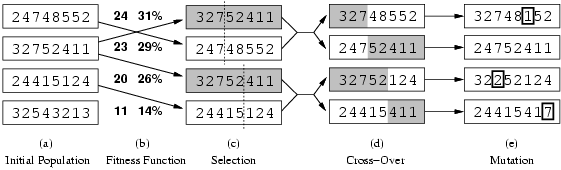
\includegraphics[width = 0.5\textwidth]{3_1.png}
\end{figure}
Local search is very useful in space exploration problem.
\clearpage
\section{Adversarial Search}
For this section, we mainly cover deterministic games.
\subsection{Game: Adversarial Search Problems}
Games is a variant of search problems but there are two unique features in games.
\begin{enumerate}
	\item Utility Maximising opponent\\
	Solution is a strategy specifying a move for every possible opponent response.
	\item Time Limit\\
	Unlikely to find goal, must approximate
\end{enumerate}
For the two-player fixed sum game, we label them as 
\begin{itemize}
	\item MAX player, who wants to maximise value
	\item MIN player, who wants to minimise value
\end{itemize}
The existence of two players with opposite goals makes the searching problem adversarial.
\begin{definition}[Game]
\hfill\\\normalfont A game is defined by 7 components:
\begin{enumerate}
	\item Initial State $s_0$
	\item States
	\item Players: \textsc{Player}($s$) defines which player has the move in state $s$.
	\item Actions: \textsc{Actions}($s$) returns set of legal moves in state $s$
	\item Transition model: \textsc{Result}($s$, $a$) returns state that results from the move $a$ in state $s$.
	\item Terminal test \textsc{Terminal}($s$) returns \texttt{true} if game is over and \texttt{false} otherise
	\item Utility function \textsc{Utility}($s$, $p$) gives final numeric value for a game that ends in terminal state $s$ for a player $p$
\end{enumerate}
\end{definition}
\begin{definition}[Constant-sum Game]
\hfill\\\normalfont A game is a constant-sum game if total utility score over all agents sum to constant.
\end{definition} 
\textbf{Remark}: Player strategy still needs to specify behaviour in states that will never be reached.
\begin{definition}[Winning/Non-losing Strategy]
\hfill\\\normalfont A strategy $s_1^\ast$ for player 1 is called \textbf{winning} if for any strategy $s_2$ by player 2, the game ends with player 1 as the winner.\\
A strategy $t_1^\ast$ for player 1 is called \textbf{non-losing} if for any strategy $s_2$ by player 2, the game ends in either a tie or a win for player 1.
\end{definition}
\begin{theorem}
\hfill\\\normalfont In the game of chess, only one of the following is true:
\begin{enumerate}
	\item White has a winning strategy $s_W^\ast$
	\item Black has a winning strategy $s_B^\ast$
	\item Each player has a non-losing strategy
\end{enumerate}
\end{theorem}
\subsection{Minimax}
\begin{definition}[Minimax]
\hfill\\\normalfont The optimal strategy at every node for the two player can be derived using the minimax algorithm, as it achieves subperfect nash equilibrium.
\[
\textsc{Minimax}(s)=\begin{cases}
\textsc{Utility}(s)&\text{ if }\textsc{Terminal}(s)\\
\max_{\alpha\in\textsc{Actions}(s)}\textsc{Minimax}(\textsc{Result}(s,a))&\text{ if }\textsc{Player}(s)=\text{MAX}\\
\min_{\alpha\in\textsc{Actions}(s)}\textsc{Minimax}(\textsc{Result}(s,a))&\text{ if }\textsc{Player}(s)=\text{MIN}
\end{cases}
\]
\end{definition}
\begin{table}[h]
\centering
\begin{tabular}{|l|l|}
\hline
Complete?&Yes(if game tree is finite)\\\hline
Optimal?&Yes\\\hline
Time&$O(b^m)$\\\hline
Space&$O(bm)$\\\hline
\end{tabular}
\end{table}
\subsection{{$\alpha-\beta$ Pruning}}
The game tree of \textsc{Minimax} algorithm is very huge in practice and $\alpha-\beta$ pruning is required to optmise the search.
\begin{definition}[{$\alpha,\beta$}]
\hfill\\\normalfont For each MAX node $n$, $\alpha(n)$ is the highest observed value found on all paths from $n$; initially $\alpha(n)=-\infty$.\\
For each MIN node $n$, $\beta(n)$ is the lowest observed value found on all paths from $n$; initially $\beta(n)=+\infty$.
\end{definition}
\begin{theorem}[Alpha/Beta Prune]
\hfill\\\normalfont \textbf{Alpha prune}: Given a MIN node $n$, stop searching below $n$ if there is some MAX ancestor $i$ of $n$ with $\alpha(i)\geq \beta(n)$.\\
\textbf{Beta prune}: Given a MAX node $n$, stop searching below $n$ if there is some MIN ancestor $i$ of $n$ with $\beta(i)\leq \alpha(n)$.
\end{theorem}
\textbf{Remark}:\\
\begin{itemize}
	\item When we prune a branch, it \textbf{never} affects final outcome.
	\item Good move ordering improves effectiveness of pruning
	\item ``Perfect'' ordering improves time complexity to $O(b^{\frac{m}{2}})$.
	\item Random ordering improves time complexity to $O(b^{\frac{3}{4}m})$ for $b<1000$.
\end{itemize}
\subsection{Evaluation Function}
$\alpha-\beta$ pruning does not resolve the problem of the large depth of the game tree.\\
Standard solution to the problem is
\begin{itemize}
	\item Evaluation function, which estimates the expected utility of the state
	\item Cutoff test, which limits the depth of the traversal
\end{itemize}
\begin{definition}[Heuristic Minimax Value]
\hfill\\\normalfont Heuristic Minimax algorithm makes uses of the evaluation function and cutoff test.
\[
\textsc{H-Minimax}(s,d)=\begin{cases}
\textsc{Eval}(s)&\text{ if }\textsc{Cutoff-Test}(s,d)\\
\max_{\alpha\in\textsc{Actions}(s)}\textsc{H-Minimax}(\textsc{Result}(s,a),d+1)&\text{ if }\textsc{Player}(s)=\text{MAX}\\
\min_{\alpha\in\textsc{Actions}(s)}\textsc{H-Minimax}(\textsc{Result}(s,a),d+1)&\text{ if }\textsc{Player}(s)=\text{MIN}
\end{cases}
\]
\end{definition}
The above algorithm will run \textsc{Minimax} until depth $d$, and use evaluation function for nodes of depth greater than $d$.
\begin{definition}[Evaluation Function]
\hfill\\\normalfont An evaluation function is a mapping from game states to real values $f:S\to \mathbb{R}$.
\end{definition}
The evaluation function should observe the following properties:
\begin{itemize}
\item Cheap to compute
\item For non-terminal states, it must be strongly \textbf{correlated} with actual chances of winning
\end{itemize}
It would be good if the evaluation function maintains the relative ordering of game states.
\begin{definition}[Modern Evaluation Functions]
\hfill\\\normalfont Modern evaluation functions are usually in the form of weighted sum of position features:
\[
f(n) = \sum_{i\in I}w_i\text{feat}_i(n)
\] 
The weights are usually determined dynamically.
\end{definition}
\textbf{Remark}: Cutting off search can be combined with iterative deepening.
\subsection{Stochastic Games}
Stochastic games are games involved with uncertainty. Minimax needs to add a chance layer for the calculated of the \textbf{expected} value of a state.
\clearpage
\section{Constraint Satisfaction Problems}
\subsection{Constraint Satisfaction Problems}
Previously, we have covered standrad search problem where state is atomic.
\begin{definition}[Constraint Satisfaction Problem]
\hfill\\\normalfont A constraint satisfaction problem consists of the following components:
\begin{itemize}
\item Variables $\mathbf{X}=(X_1,\ldots, X_n)$; each variable $X_i$ has a domain $D_i$.
\item Constraints $\mathbf{C}$, which involves
\begin{itemize}
	\item Constraint scope: which variables are involved
	\item Constraint relation: what is the relation between them
\end{itemize}
\item Objective: find a legal assignment $(y_1,\ldots, y_n)$ of values to variables $(X_1,\ldots, X_n)$, such that
\begin{itemize}
	\item $y_i\in D_i$ for all $i\in[n]$.
	\item Constraints are all satisfied.
\end{itemize}
\end{itemize}
\end{definition}
Constraint satisfaction problem(CSP) is a broad modelling framework. Examples of CSP include graph coloring and job-shop scheduling.\\
Different aspects of CSP include
\begin{itemize}
\item Discrete variables of finite domains and infinite domains \textbf{vs} continuous variables
\item Unary constraints \textbf{vs} Binary constraints \textbf{vs} Global(i.e. higher-oredr) constraints
\end{itemize} 
CSP can be solved using standard search formulation:
\begin{itemize}
	\item Each state is a partial variable assignment
	\item \textbf{Initial State}: the empty assignment $[]$
	\item \textbf{Transition Function}: assign a \textit{valid} value to an unassigned variable; fail if no \textit{valid} assignments
	\item \textbf{Goal Test}: all variables have been assigned.
\end{itemize}
One very useful properties of CSP is that \textit{every} solution appears at depth $n$, where $n$ variables have been assigned. Therefore, the best search technique is DFS.\\
\begin{definition}[Backtracking Search]
\hfill\\\normalfont DFS for CSPs with single-variable assignment is called \textbf{backtracking search}. It performs backtracking when there is no legal assignments before reaching any goal.\\
\textbf{function} \textsc{Backtracking-Search}(\textit{csp}) \textbf{returns} a solution, or failure\\
\ind \textbf{return} \textsc{Backtrack}($\{\}$, \textit{csp})\\
\textbf{function} \textsc{Backtrack}(\textit{assignment}, \textit{csp}) \textbf{returns} a solution, or failure\\
\ind \textbf{if} \textit{assignment} is complete \textbf{then return} \textit{assignment}\\
\ind \textit{var}$\leftarrow$\textsc{Select-Unassigned-Variable}(\textit{csp})\\
\ind \textbf{for each} \textit{value} \textbf{in} \textsc{Order-Domain-Values}(\textit{var}, \textit{assignment}, \textit{csp}) \textbf{do}\\ 
\ind \ind \textbf{if} \textit{value} is consistent with \textit{assignment} \textbf{then}\\
\ind \ind \ind add $\{\textit{var} = \textit{value}\}$ to \textit{assignment}\\
\ind \ind \ind \textit{inferences}$\leftarrow$\textsc{Inference}(\textit{csp}, \textit{var}, \textit{value})\\
\ind \ind \ind \textbf{if} \textit{inferences}$\neq$\textit{failure} \textbf{then}\\
\ind \ind \ind \ind add \textit{inferences} to \textit{assignment}\\
\ind \ind \ind \ind \textit{result}$\leftarrow$\textsc{Backtrack}(\textit{assignment}, \textit{csp})\\
\ind \ind \ind \ind \textbf{if} \textit{result}$\neq$\textit{failure} \textbf{then}\\
\ind \ind \ind \ind \ind \textbf{return} \textit{result}\\
\ind \ind remove $\{\textit{var}=\textit{value}\}$ and \textit{inferences} from \textit{assignment}\\
\ind \textbf{return} \textit{failure}
\end{definition}
\subsection{General Purpose Heuristics}
To improve backtracking efficiency, we utilise general-purpose heuristics.
\subsubsection{Most Constrained Variable}
This strategy, a.k.a. minimum-remaining-values(MRV) heuristic, chooses the variable with \textit{fewest legal} values.
\subsubsection{Most Constraining Variable}
This strategy, a.k.a. degree heuristic, chooses the variable with most constraints on remaining unassigned variables.
\subsubsection{Least Constraining Value}
This strategy, given a variable, chooses the least constraining value. Equivalently, it chooses te one value that rules out the fewest values for the neighbouring unassigned variables.
\subsection{Forward Checking}
Forward checking works by
\begin{itemize}
	\item Keep track of remaining legal values for unassigned variables
	\item Terminate search when any variable has no legal values
\end{itemize}
Despite forward checking propogates information from assigned to unassigned variables, it does not necessarily provide early detections for all failures.
\subsection{Constraint Propagation}
Constraint propagation improves on forward checking, by repeatedly locally enforces constraints.\\Constraint propagation generate inferences in CSPs by looking at
\begin{itemize}
	\item Node consistency for unary constraints
	\item Arc consistency for binary constraints
	\item Other constraints
\end{itemize}
Constraint propagation can be either interleaved with search, or run as a preprocessing step.
\subsubsection{Arc Consistency}
Simplest form of propagation will make each arc consistent.
\begin{definition}[Arc Consistent]
\hfill\\\normalfont $X_i$ is arc-consistent with respect to $X_j$ if and only if for every value $x\in D_i$, there exists some value $y\in D_j$ that satisfies the binary constraint on the arc $(X_i, X_j)$.
\end{definition}
The propagation by arc consistency works by looking at the updated codomain, and trims the domain until no elements in teh domain maps outside the updated codomain. \\
This will usually cause a chain reaction, and it detects failure earlier than forward checking.
\begin{theorem}[Arc Consistency Algorithm AC-3]
\hfill\\\normalfont
\textbf{function} AC-3(\textit{csp}) \textbf{returns} false if an inconsistency is found and true otherwise\\
\ind \textbf{inputs}: \textit{csp}, a binary CSP with components $(X,D,C)$\\
\ind \textbf{local variables}: \textit{queue}, a queue of arcs, initially all the arcs in \textit{csp}\\

\ind \textbf{while} \textit{queue} is not empty \textbf{do}\\
\ind \ind $(X_i, X_j)\leftarrow$ \textsc{Remove-First}(\textit{queue})\\
\ind \ind \textbf{if} \textsc{Revise}(\textit{csp}, $X_i$, $X_j$) \textbf{then}\\
\ind \ind \ind \textbf{if} size of $D_i=0$ \textbf{then return} \textit{false}\\
\ind \ind \ind \textbf{for each} $X_k$ \textbf{in} $X_i$.\textsc{Neighbours}$-\{X_j\}$ \textbf{do}\\
\ind \ind \ind \ind add $(X_k,X_i)$ to \textit{queue}\\
\ind \textbf{return} \textit{true}

\textbf{function} \textsc{Revise}(\textit{csp}, $X_i$, $X_j$) \textbf{returns} true iff we revise the domain of $X_i$\\
\ind \textit{revised}$\leftarrow$ \textit{false}\\
\ind \textbf{for each} $x$ \textbf{in} $D_i$ \textbf{do}\\
\ind \ind \textbf{if} no value $y$ in $D_j$ allows $(x, y)$ to satisfy the constraint between $X_i$ and $X_j$ \textbf{then}\\
\ind \ind \ind delete $x$ from $D_i$\\
\ind \ind \ind \textit{revised}$\leftarrow$ \textit{true}\\
\ind \textbf{return} \textit{revised}
\end{theorem}
The above algorithm gives time complexity of $O(n^2d^3)$, as
\begin{itemize}
	\item CSP has at most $n^2$ directed arcs
	\item each arc can be inserted at most $d$ times, as $X_i$ has at most $d$ values to delete
	\item Checking the consistency of an arc takes $O(d^2)$ times.
\end{itemize}
To maintain Arc Consistency, we can proceed the search as follows:
\begin{itemize}
	\item Establish AC at the root
	\item When AC-3 terminates, choose a new variable
	\item re-establish AC given the new variable choice(Maintain AC)
	\item repeat;;
	\item backtrack if AC gives \textit{empty} domain
\end{itemize}
\subsubsection{{$k$-consistency}}
Arc consistency on binary constraints can be generalised to $k$ consistency on global constraints. However, $k$ consistency need to consider not only pairwise constraints, but also constraints of more variables.
\subsection{Local Search for CSPs}
Hill-climbing, simulated annealing can be modified to be applied to CSP, by
\begin{itemize}
	\item allow states that violate constraints
	\item operators reassign variable values
\end{itemize}
The the variable value selection, we apply the \textbf{min-conflict} heuristic, which chooses value that violates the fewest constraints.
\begin{theorem}[Min-Conflict Algorithm]
\hfill\\\normalfont 
\textbf{function} \textsc{Min-Conflict}(\textit{csp}, \textit{max\_steps}) \textbf{returns} a solution or failure\\
\ind \textbf{inputs}: \textit{csp}, a constraint satisfaction problem\\
\ind \ind \ind \textit{max\_steps}, the number of steps allowed before giving up\\

\ind \textit{current}$\leftarrow$ an initial complete assignment for \textit{csp}\\
\ind \textbf{for} $i=1$ to \textit{max\_steps} \textbf{do}\\
\ind \ind \textbf{if} \textit{current} is a solution for \textit{csp} \textbf{then return} \textit{current}\\
\ind \ind \textbf{var}$\leftarrow$ a randomly chosen conflicted variable from \textit{csp}.\textsc{Variables}\\
\ind \ind \textbf{value}$\leftarrow$ the value $v$ for \textit{var} that minimises \textsc{Conflicts}(\textit{var}, \textit{v}, \textit{current}, \textit{csp})\\
\ind \ind set \textit{var}$=$\textit{value} in \textbf{current}\\
\ind \textbf{return} \textit{failure}
\end{theorem}
\clearpage
\section{Logical Agents}
\subsection{Knowledge-based Agents}
\textbf{Knowledge-based} agents represent agent domain knowledge using logical formulas. 
\begin{itemize}
	\item The central component of a knowledge-based agent is its \textbf{knowledge base} (KB), which is a set of sentences.
	\item Each sentence is expressed in a \textbf{knowledge representation language}.
	\item Declarative approach to build an agent by \textsc{Tell} it what it needs to know
	\item Then it infers by \textsc{Asking} itself what to do, from knowledge in the KB
	\item The agent must be able to 
	\begin{itemize}
		\item Represent states, actions, etc.
		\item Incorporate new percepts
		\item Update internal world representations
		\item Deduce hidden world properties, and deduce actions
	\end{itemize}
\end{itemize}
The following algorithm is one general algorithm for Knowledge Based Agents:\\
\textbf{function} \textsc{KB-agent}(\textit{percept}) \textbf{returns} an \textit{action}\\
\ind \textbf{persistent}: \textit{KB}, knowledge base \\
\ind \ind \ind \ind $t$, a counter, initially 0, indicating time\\

\ind \textsc{Tell}(\textit{KB}, \textsc{Make-Percept-Sentence}(\textit{percept}, $t$))\\
\ind \textit{action}$\leftarrow$ \textsc{Ask}(\textit{KB}, \textsc{Make-Action-Query}($t$))\\
\ind \textsc{Tell}(\textit{KB}, \textsc{Make-Action-Sentence}(\textit{action}, $t$))\\
\ind $t\leftarrow t+1$\\
\ind \textbf{return} \textit{action}
\subsection{Logic in Genral: Models and Entailment}
Following are some terms used in logic:
\begin{itemize}
	\item \textbf{Logic}: formal language for KB, infer conclusions
	\item \textbf{Syntax}: defines the sentences in the language
	\item \textbf{Semantics}: define the ``meaning'' of sentences
\end{itemize}
\begin{definition}[Modelling]
\hfill\\\normalfont $m$ models $\alpha$ if $\alpha$ is true under $m$.\\
Usually, we let $M(\alpha)$ denote the set of all models for $\alpha$.
\end{definition}
\begin{definition}[Entailment]
\hfill\\\normalfont Entailment means that one thing \textbf{follows from} another. Formally,
\[
\alpha\models \beta \Leftrightarrow M(\alpha)\subseteq M(\beta)
\]
\end{definition}
\begin{definition}[Inference]
\hfill\\\normalfont We use $KB\vdash_i\alpha$ to mean ``sentence $\alpha$ is derived from KB by inference algorithm $i$''.\\
\begin{itemize}
	\item \textbf{Soundness}: $i$ is sound if $KB\vdash_i\alpha$ implies $KB\models \alpha$.
	\item \textbf{Completeness}: $i$ is complete if $KB\models \alpha$ implies $KB\vdash_i\alpha$.
\end{itemize}
\end{definition}
Inference is done by deriving knowledge out of percepts. Specifically, given $KB$ and $\alpha$, we want to know if $KB\vdash \alpha$.
\subsection{Propositional Logic}
\subsubsection{Syntax}
Sentence in propositional logic are represented by symbols, like $S_i$. Logical connectives are used to construct complex sentences from simpler ones:
\begin{itemize}
	\item If $S$ is a sentence, $\neg S$ is a sentence.
	\item If $S_1, S_2$ are sentences,
	\begin{itemize}
		\item $S_1\land S_2$ is a sentence.
		\item $S_1\lor S_2$ is a sentence.
		\item $S_1\Rightarrow S_2$ is a sentence.
		\item $S_1\Leftrightarrow S_2$ is a sentence.
	\end{itemize}
\end{itemize}
\subsubsection{Semantics}
A model is a \textbf{truth assignment} to the basic variables. All other sentences' truth value is derived according to logical rules.
\subsubsection{Inference by Truth Table Enumeration}
We adopt depth-first enumeration of all models. This guarantees soundness and completeness.\\
For $n$ symbols, time complexity is $O(2^n)$ and space complexity is $O(n)$.\\
Below is the algorithm:\\
\textbf{function} \textsc{TT-Entails?}(\textit{KB}, $\alpha$) \textbf{returns} \textit{true} or \textit{false}\\
\ind \textbf{inputs}: \textit{KB}, the knowledge base, a sentence is propositional logic\\
\ind \ind \ind $\alpha$, the query, a sentence in propositional logic\\

\ind \textit{symbols}$\leftarrow$ a list of the proposition symbols in \textit{KB} and $\alpha$
\ind \textbf{return} \textsc{TT-Check-All}(\textit{KB}, $\alpha$, \textit{symbols}, $\{\}$)\\

\textbf{function} \textsc{TT-Check-All}((\textit{KB}, $\alpha$, \textit{symbols}, \textit{model}) \textbf{returns} \textit{true} or \textit{false}\\
\ind \textbf{if} \textsc{Empty?}(\textit{symbols}) \textbf{then}\\
\ind \ind \textbf{if} \textsc{PL-True?}(\textit{KB}, \textit{model}) \textbf{then return} \textsc{PL-True?}($\alpha$, \textit{model})\\
\ind \ind \textbf{else return} \textit{true}\\
\ind \textbf{else do}\\
\ind \ind $P\leftarrow$\textsc{First}(\textit{symbols})\\
\ind \ind \textit{rest}$\leftarrow$\textsc{Rest}(\textit{symbols})\\
\ind \ind \textbf{return} (\textsc{TT-Check-All}(\textit{KB}, $\alpha$, \textit{rest}, \textit{model}$\cup\{P=\textit{true}\}$)\\
\ind \ind \ind \ind \textbf{and}\\
\ind \ind \ind \ind \textsc{TT-Check-All}(\textit{KB}, $\alpha$, \textit{rest}, \textit{model}$\cup\{P=\textit{false}\}$)

\subsection{Equivalence, Validity, Satisfiability}
\begin{definition}[Validity]
\hfill\\\normalfont A sentence is \textbf{valid} if it is true in \textit{all} models.
\end{definition}
\begin{theorem}[Deduction Theorem]
\hfill\\\normalfont Validity is connected to entailment through deduction theorem:
\[
KB\models \alpha\Leftrightarrow (KB\Rightarrow \alpha) \text{ is valid}
\]
\end{theorem}
\begin{definition}[Satisfiability]
\hfill\\\normalfont A sentence is satisfiable if it is true in \textbf{some} model.\\
A sentencxe is unsatisfiable if it is true in \textit{no} models.
\end{definition}
\begin{theorem}[Satisfiability and entailment]
\hfill\\\normalfont Satisfiability is connected to entailment via the following:
\[
KB\models \alpha \Leftrightarrow (KB\land \neg \alpha) \text{ is unsatisfiable}
\]
\end{theorem}
\subsection{Proof Methods}
There are two ways of proving an proposition, either by applying inference rules, or by model checking.\\
Examples of inference rules include 
\begin{itemize}
	\item And elimination: $a\land b\models a$.
	\item Modus Ponens: $a\land (a\Rightarrow b)\models b$.
	\item Logical Equivalence: $(a\lor b)\models \neg(\neg a\land \neg b)$.
\end{itemize}
\subsubsection{Resolution for Conjunctive Normal Form}
Suppose we have a conjunction of disjunction of literals(clauses), and if a literal $x$ appeas in $C_1$ and its negation $\neg x$ in $C_2$, it can be resolved as:
\[
\frac{(x_1\lor \cdots \lor x_m\lor x)\land (y_1\lor \cdots \lor y_n\lor \neg x)}{(x_1\lor \cdots \lor x_m\lor y_1\lor \cdots \lor y_n)}
\]
Resolution is sound and complete for propositional logic.
\end{document}